\documentclass{article}

%================  CUSTOMIZATION  =================================================%

\usepackage{../KjelsethReportStyle}

%================  METADATA  ======================================================%

\title{\fontsize{24}{36}\selectfont Elektroniske enheter og kretser\\ % Input title
Lab 01} % Line 2 of title, \\ means next line.

\author{{\ttfamily Sølve Kjelseth}} % Input your name.
% replace \ttfamily with \normalfont to make it regular font.
% (removing \ttfamily will not do this automatically.

\date{\today} % Auto updates the date, until you export it.


%================  START OF DOCUMENT  =============================================%

\begin{document}

\maketitle % Makes title front page based on the title, author and date metadata, change at the top

%================  INTRODUCTION  ==================================================%

% #region introduction
\addtocontents{toc}{\protect\setcounter{tocdepth}{0}} % Temporarily hide from TOC
\section{Introduction} % Numbered section named Introduction
This is the first report in this course, detailing the completion of the first lab exercise.\par
\vfill
Note: As always, the \LaTeX\ file and all other assets, such as text, images, graphs and code made by me for this project is open source with the MIT licence, see
\linkgithub[true][0.5]{my GitHub}

\clearpage

\tableofcontents % Generate TOC
\hfill
\listoffigures % List of figures
\hfill
\listoftables % List of tables
\addtocontents{toc}{\protect\setcounter{tocdepth}{2}} % Restore TOC depth
% #endregion

%================  SECTION  =======================================================%

\section{Part 1 - Diode test}
% #region
This Part is about testing a diode characteristics with a multimeter. This means it is inherently not perfect, but it will function as a reference measurment.

%================  SINGLE FIGURE  =================================================%

\begin{figure}[h]
    \centering
    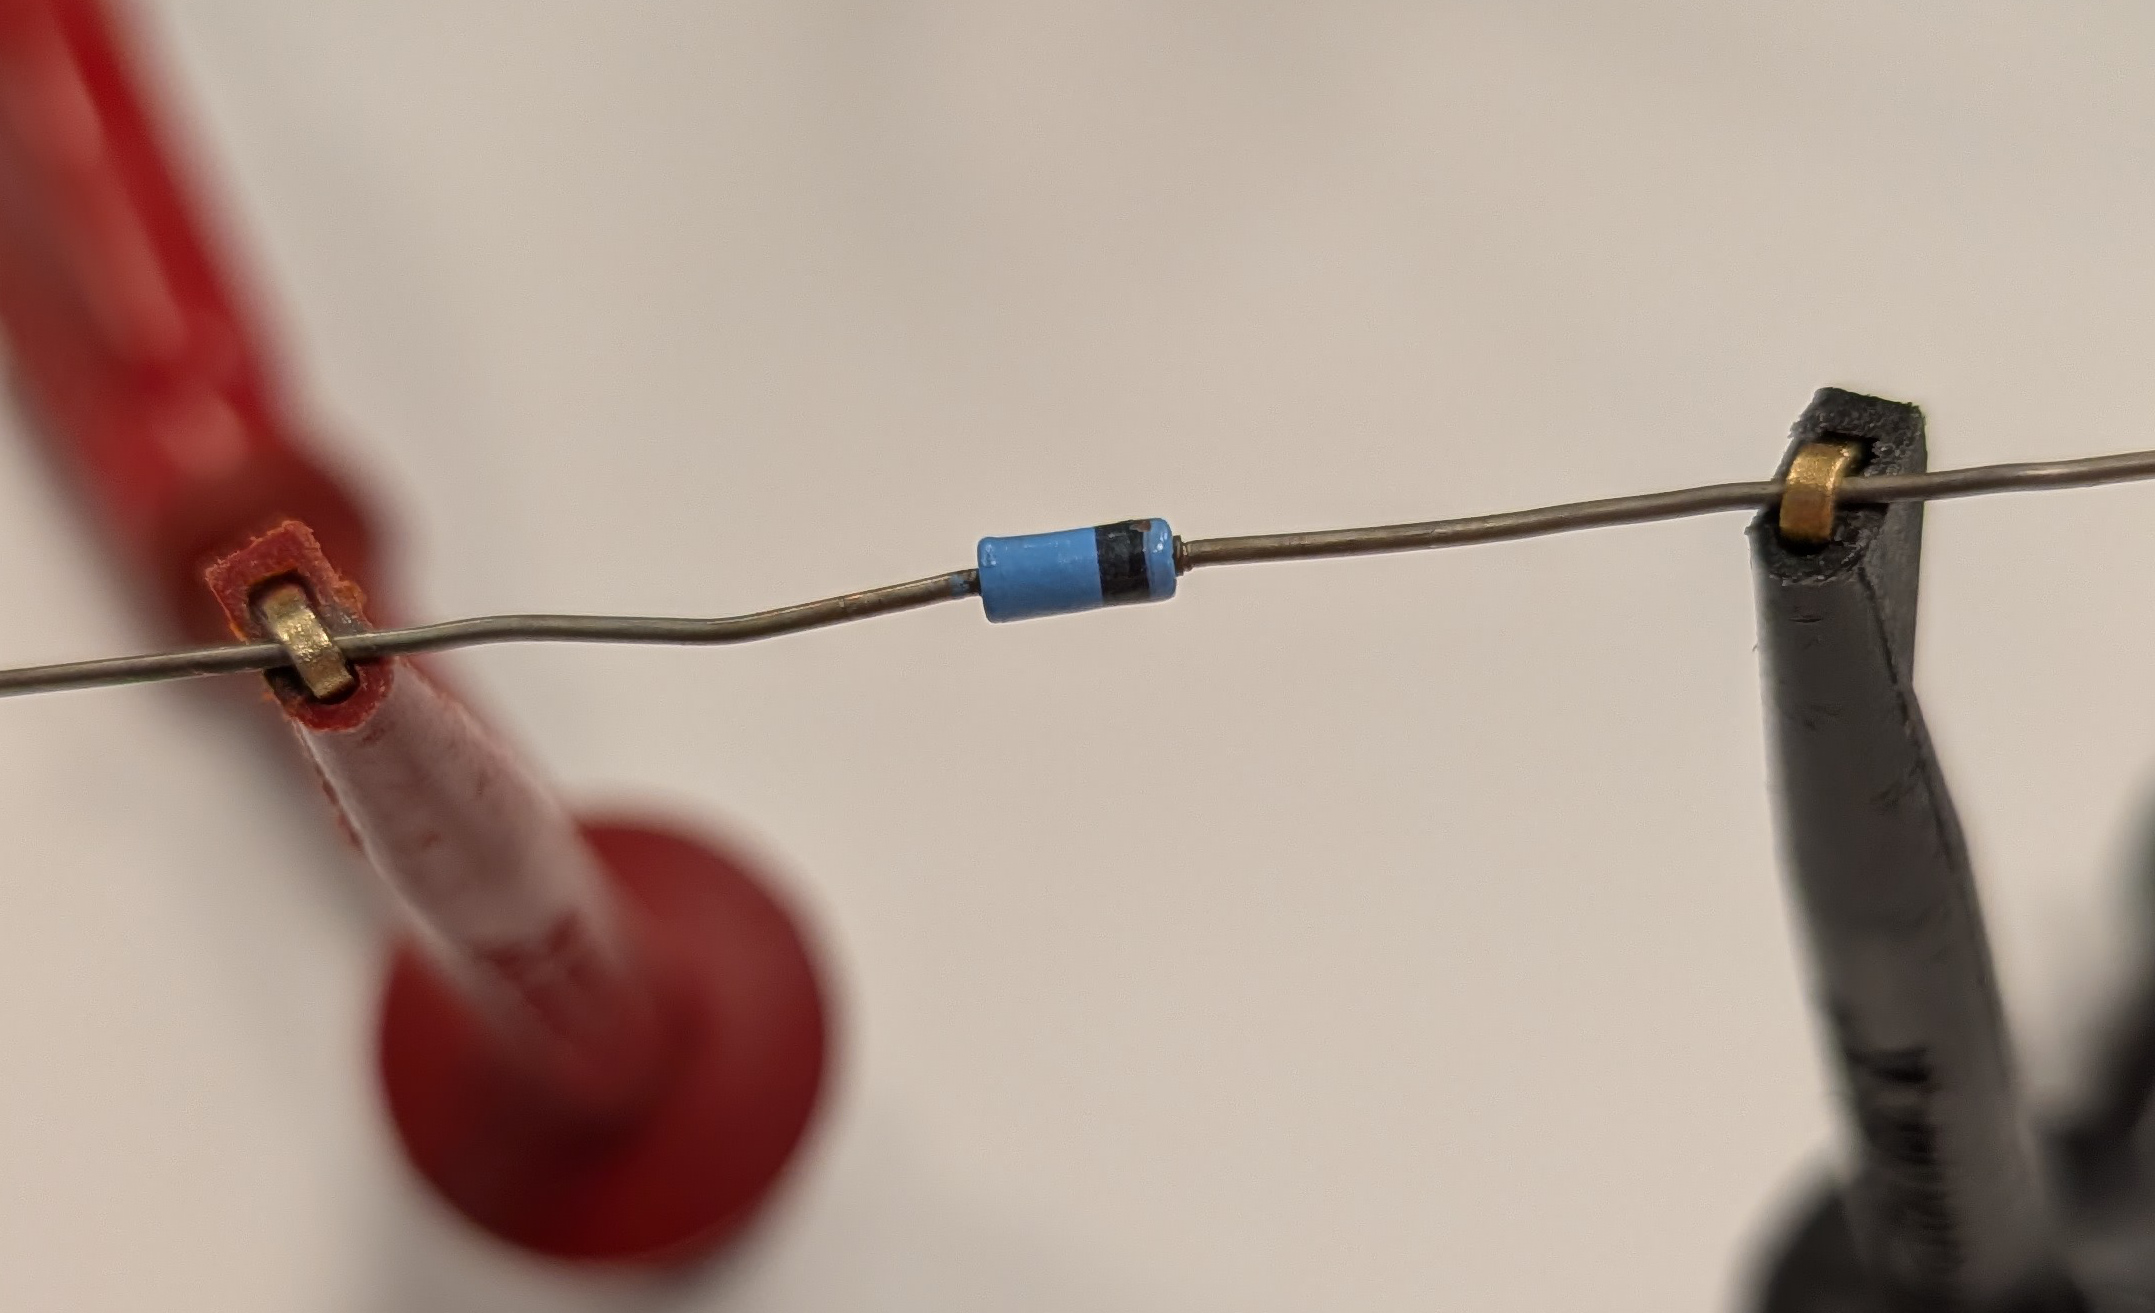
\includegraphics[width=\textwidth]{Part1.jpg}
    \caption{Diode being measured}
    \label{fig:part1}
\end{figure}

%================  TABLE  =========================================================%

% Table generated by Excel2LaTeX from sheet 'Sheet1'
\begin{table}[htbp]
  \centering
  \caption{Diode measurments}
    \begin{tabular}{|l|lr|l|lr|}
    \hline
    Voltage forward & \multicolumn{1}{r}{0.593} & \multicolumn{1}{l|}{V} & Resistance forward & \multicolumn{1}{r}{225400} & \multicolumn{1}{l|}{\Omega} \bigstrut\\
    \hline
    Voltage reverse & OL    &       & Resistance reverse & OL    &  \bigstrut\\
    \hline
    \end{tabular}%
  \label{tab:part1}%
\end{table}%


Interesting to note that the measured resistance in forward-bias of the diode fluctuated a lot. It went into high \(\SI{}{\mega\ohm}\) to low tens of \(\SI{}{\kilo\ohm}\). It was most stable around \(\SI{200}{\kilo\ohm}\) and one of these measurmens was therfore noted down. This could be because the multimeter is acting as a powersupply in resistance measuring mode and depending on the voltage chosen by the autoranging multimeter the diode behaviour differs.
% #endregion

%================  SECTION  =======================================================%

\section{Part 2 - Forward-bias characteristics}
% #region
This Part is about testing the diode characteristics for forward-bias. The values was stored in a table (RAW data like this is found on the \linkgithub{GitHub}) and then a plot was made to compare the current through the diode \(I_D\) with the voltage drop over the diode \(V_D\).

%================  SINGLE FIGURE  =================================================%

\begin{figure}[h]
    \centering
    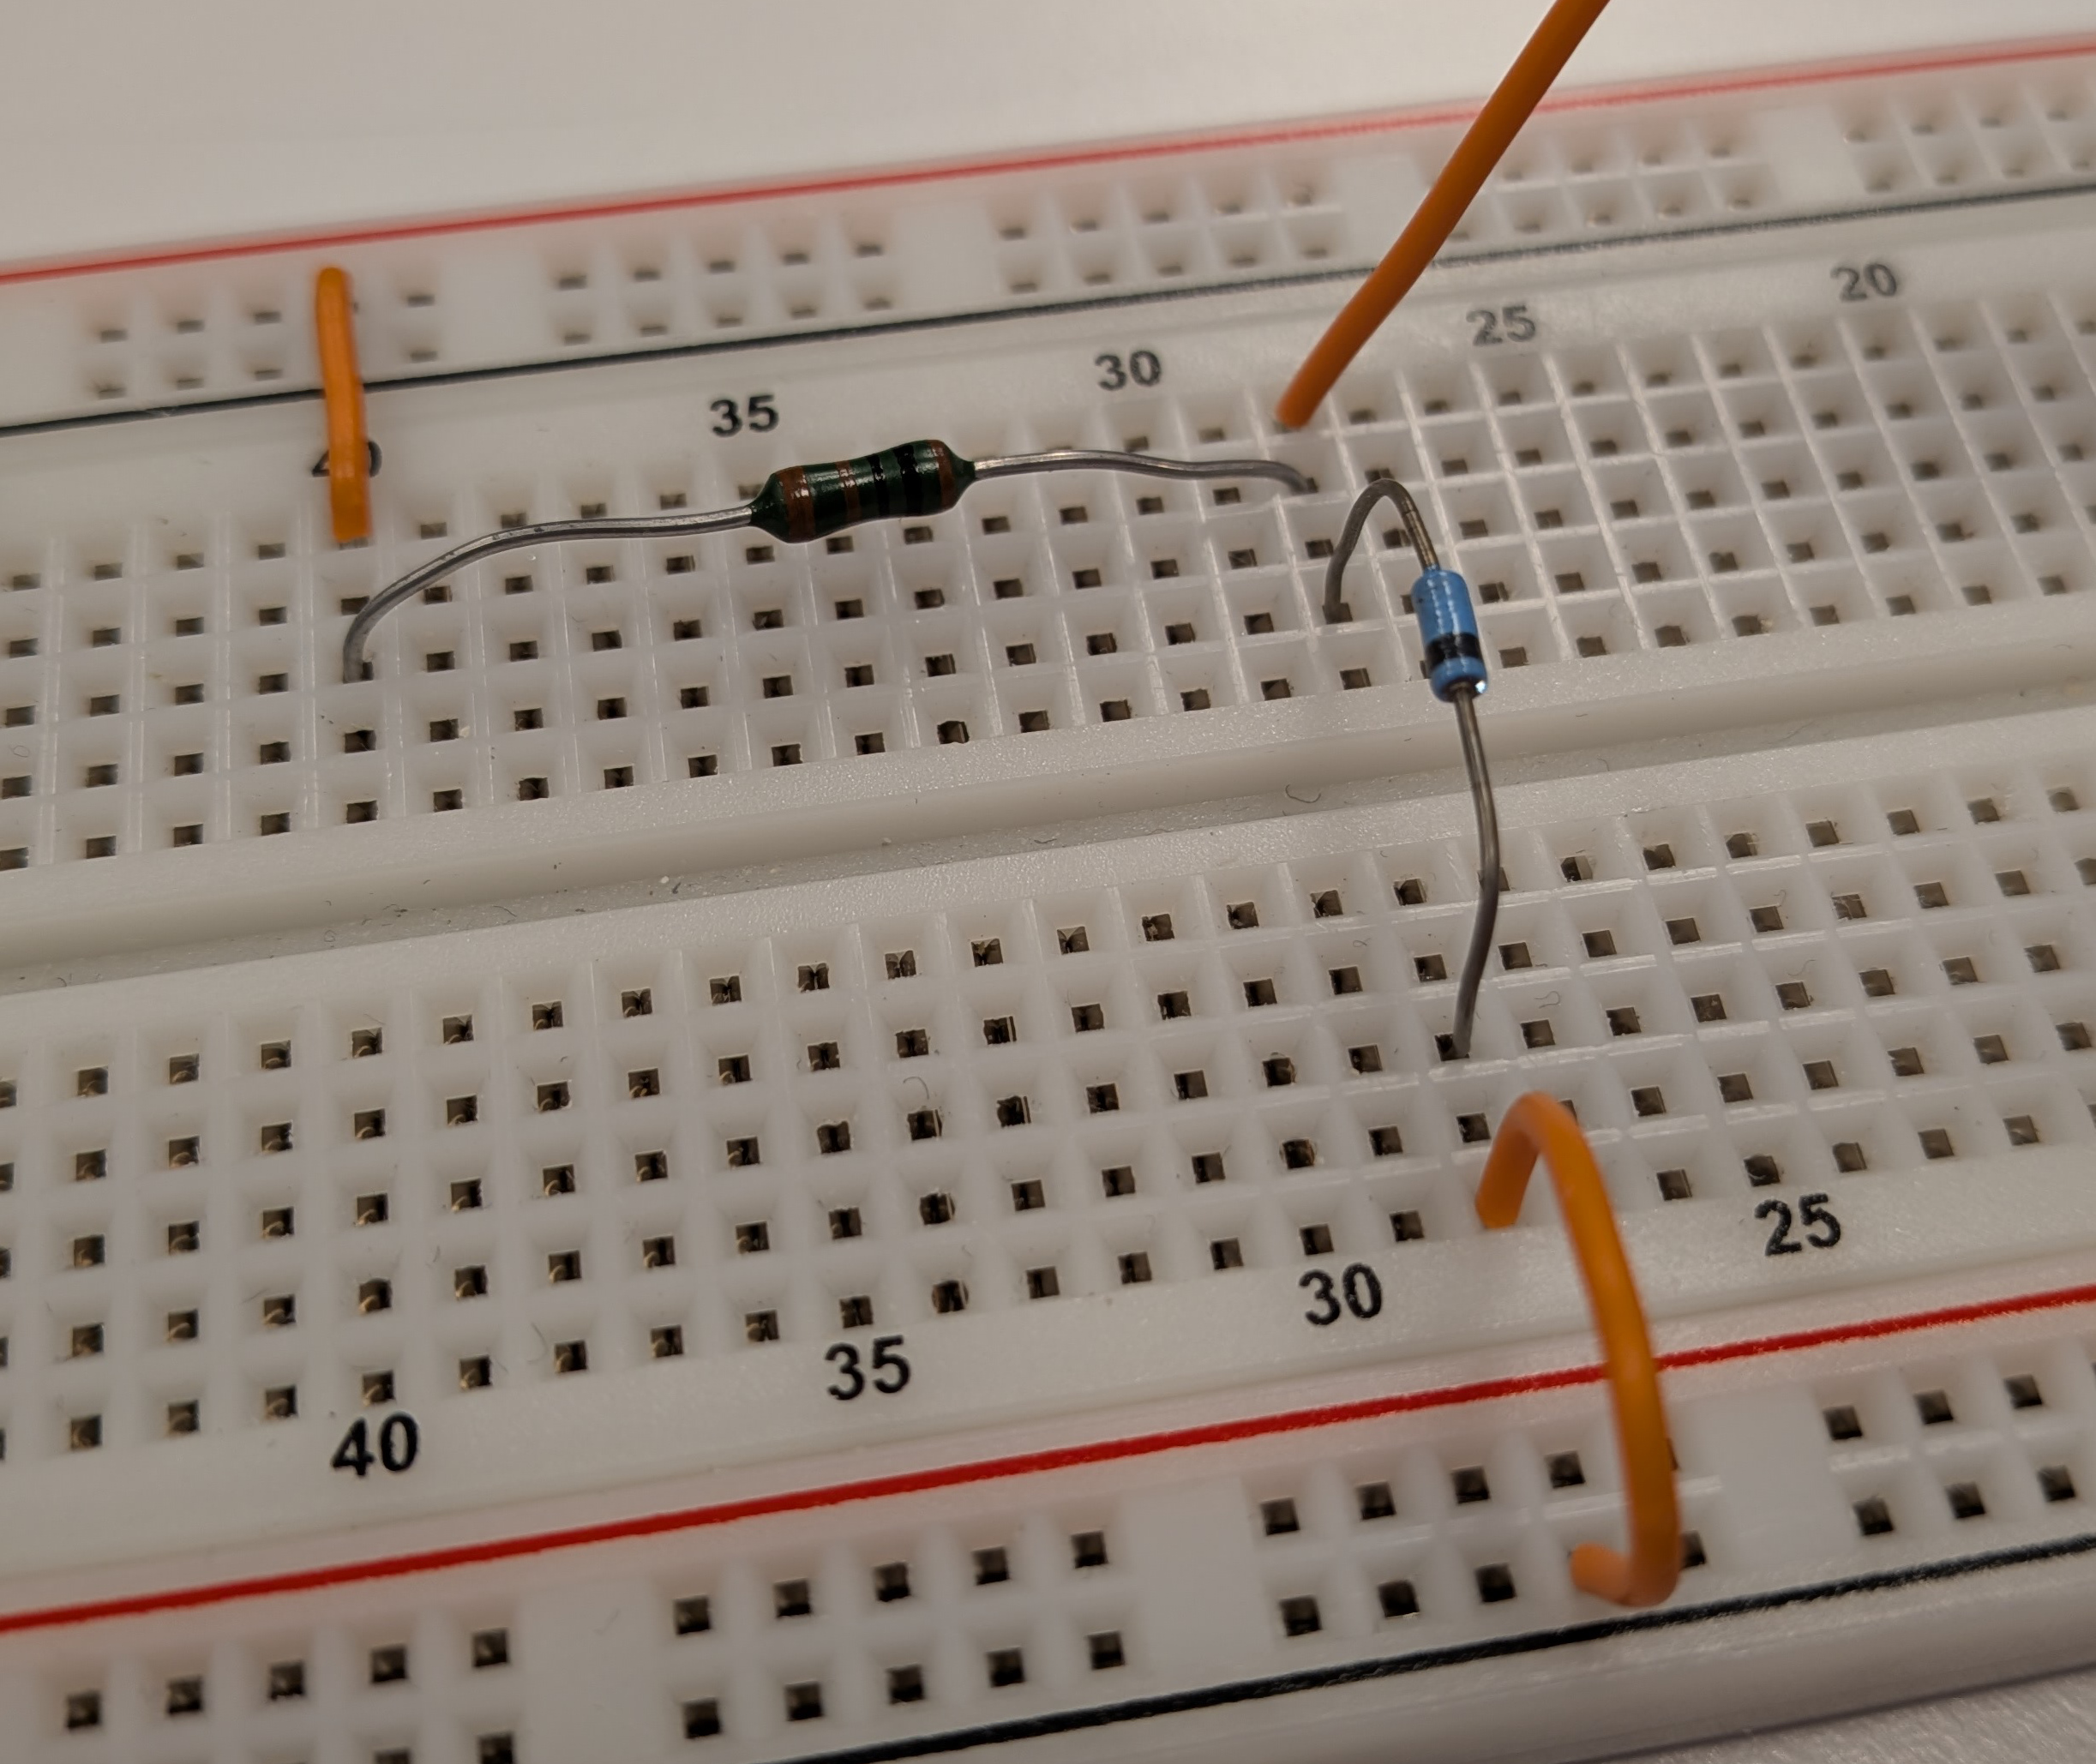
\includegraphics[width=\textwidth]{Part2.jpg}
    \caption{Part 2 circuit}
    \label{fig:Part2}
\end{figure}

\clearpage

%================  SINGLE FIGURE  =================================================%

\begin{figure}[h]
    \centering
    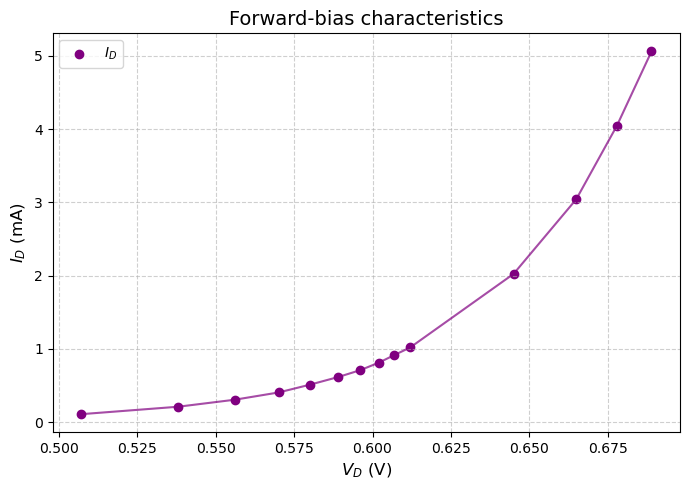
\includegraphics[width=\textwidth]{Part2Plot.png}
    \caption{Plot of forward-bias characteristics}
    \label{fig:Part2Plot}
\end{figure}

Now when when extending the plot all the way to the origin it gets a characteristics that looks a lot different. As seen in Figure~\ref{fig:Part2PlotExtended} it looks like after the initial curve the value gets linear.

\clearpage

%================  SINGLE FIGURE  =================================================%

\begin{figure}[h]
    \centering
    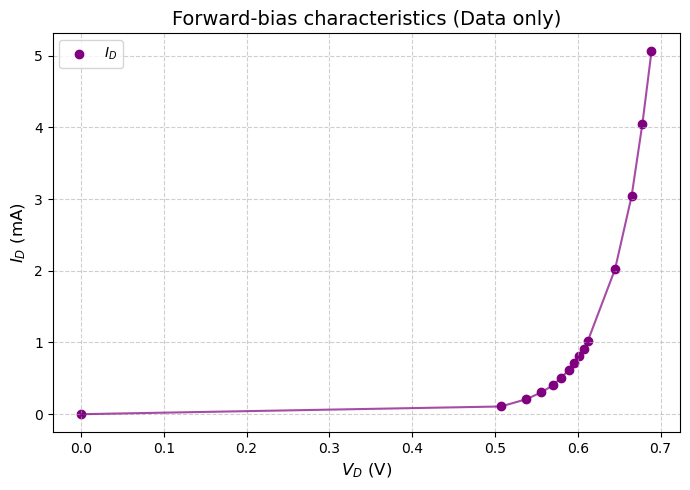
\includegraphics[width=\textwidth]{Part2PlotExtended.png}
    \caption{Extended plot of forward-bias characteristics}
    \label{fig:Part2PlotExtended}
\end{figure}

This looks now very much like an exponential relationship, when checked, the end result is very similar to to this function. This shows that the behaviour can be very accurately modelled easily using the exponential function.

\clearpage

%================  SINGLE FIGURE  =================================================%

\begin{figure}[h]
    \centering
    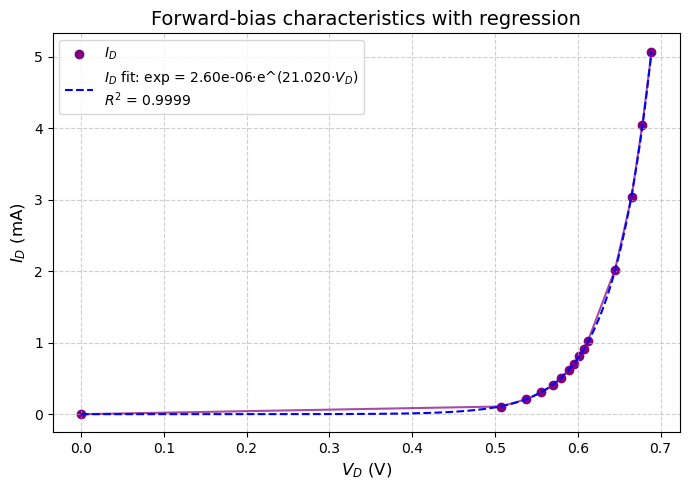
\includegraphics[width=\textwidth]{Part2PlotExp.png}
    \caption{Extended plot with exponential regression}
    \label{fig:Part2PlotExp}
\end{figure}

% #endregion

%================  SECTION  =======================================================%

\section{Part 3 - Reverse-bias}
% #region
This Part is about testing the reverse-bias current. Measurments was made and noted in the table, note that the assumed resistive value of the voltmeter is specified by the assignment.

%================  SINGLE FIGURE  =================================================%

\begin{figure}[h]
    \centering
    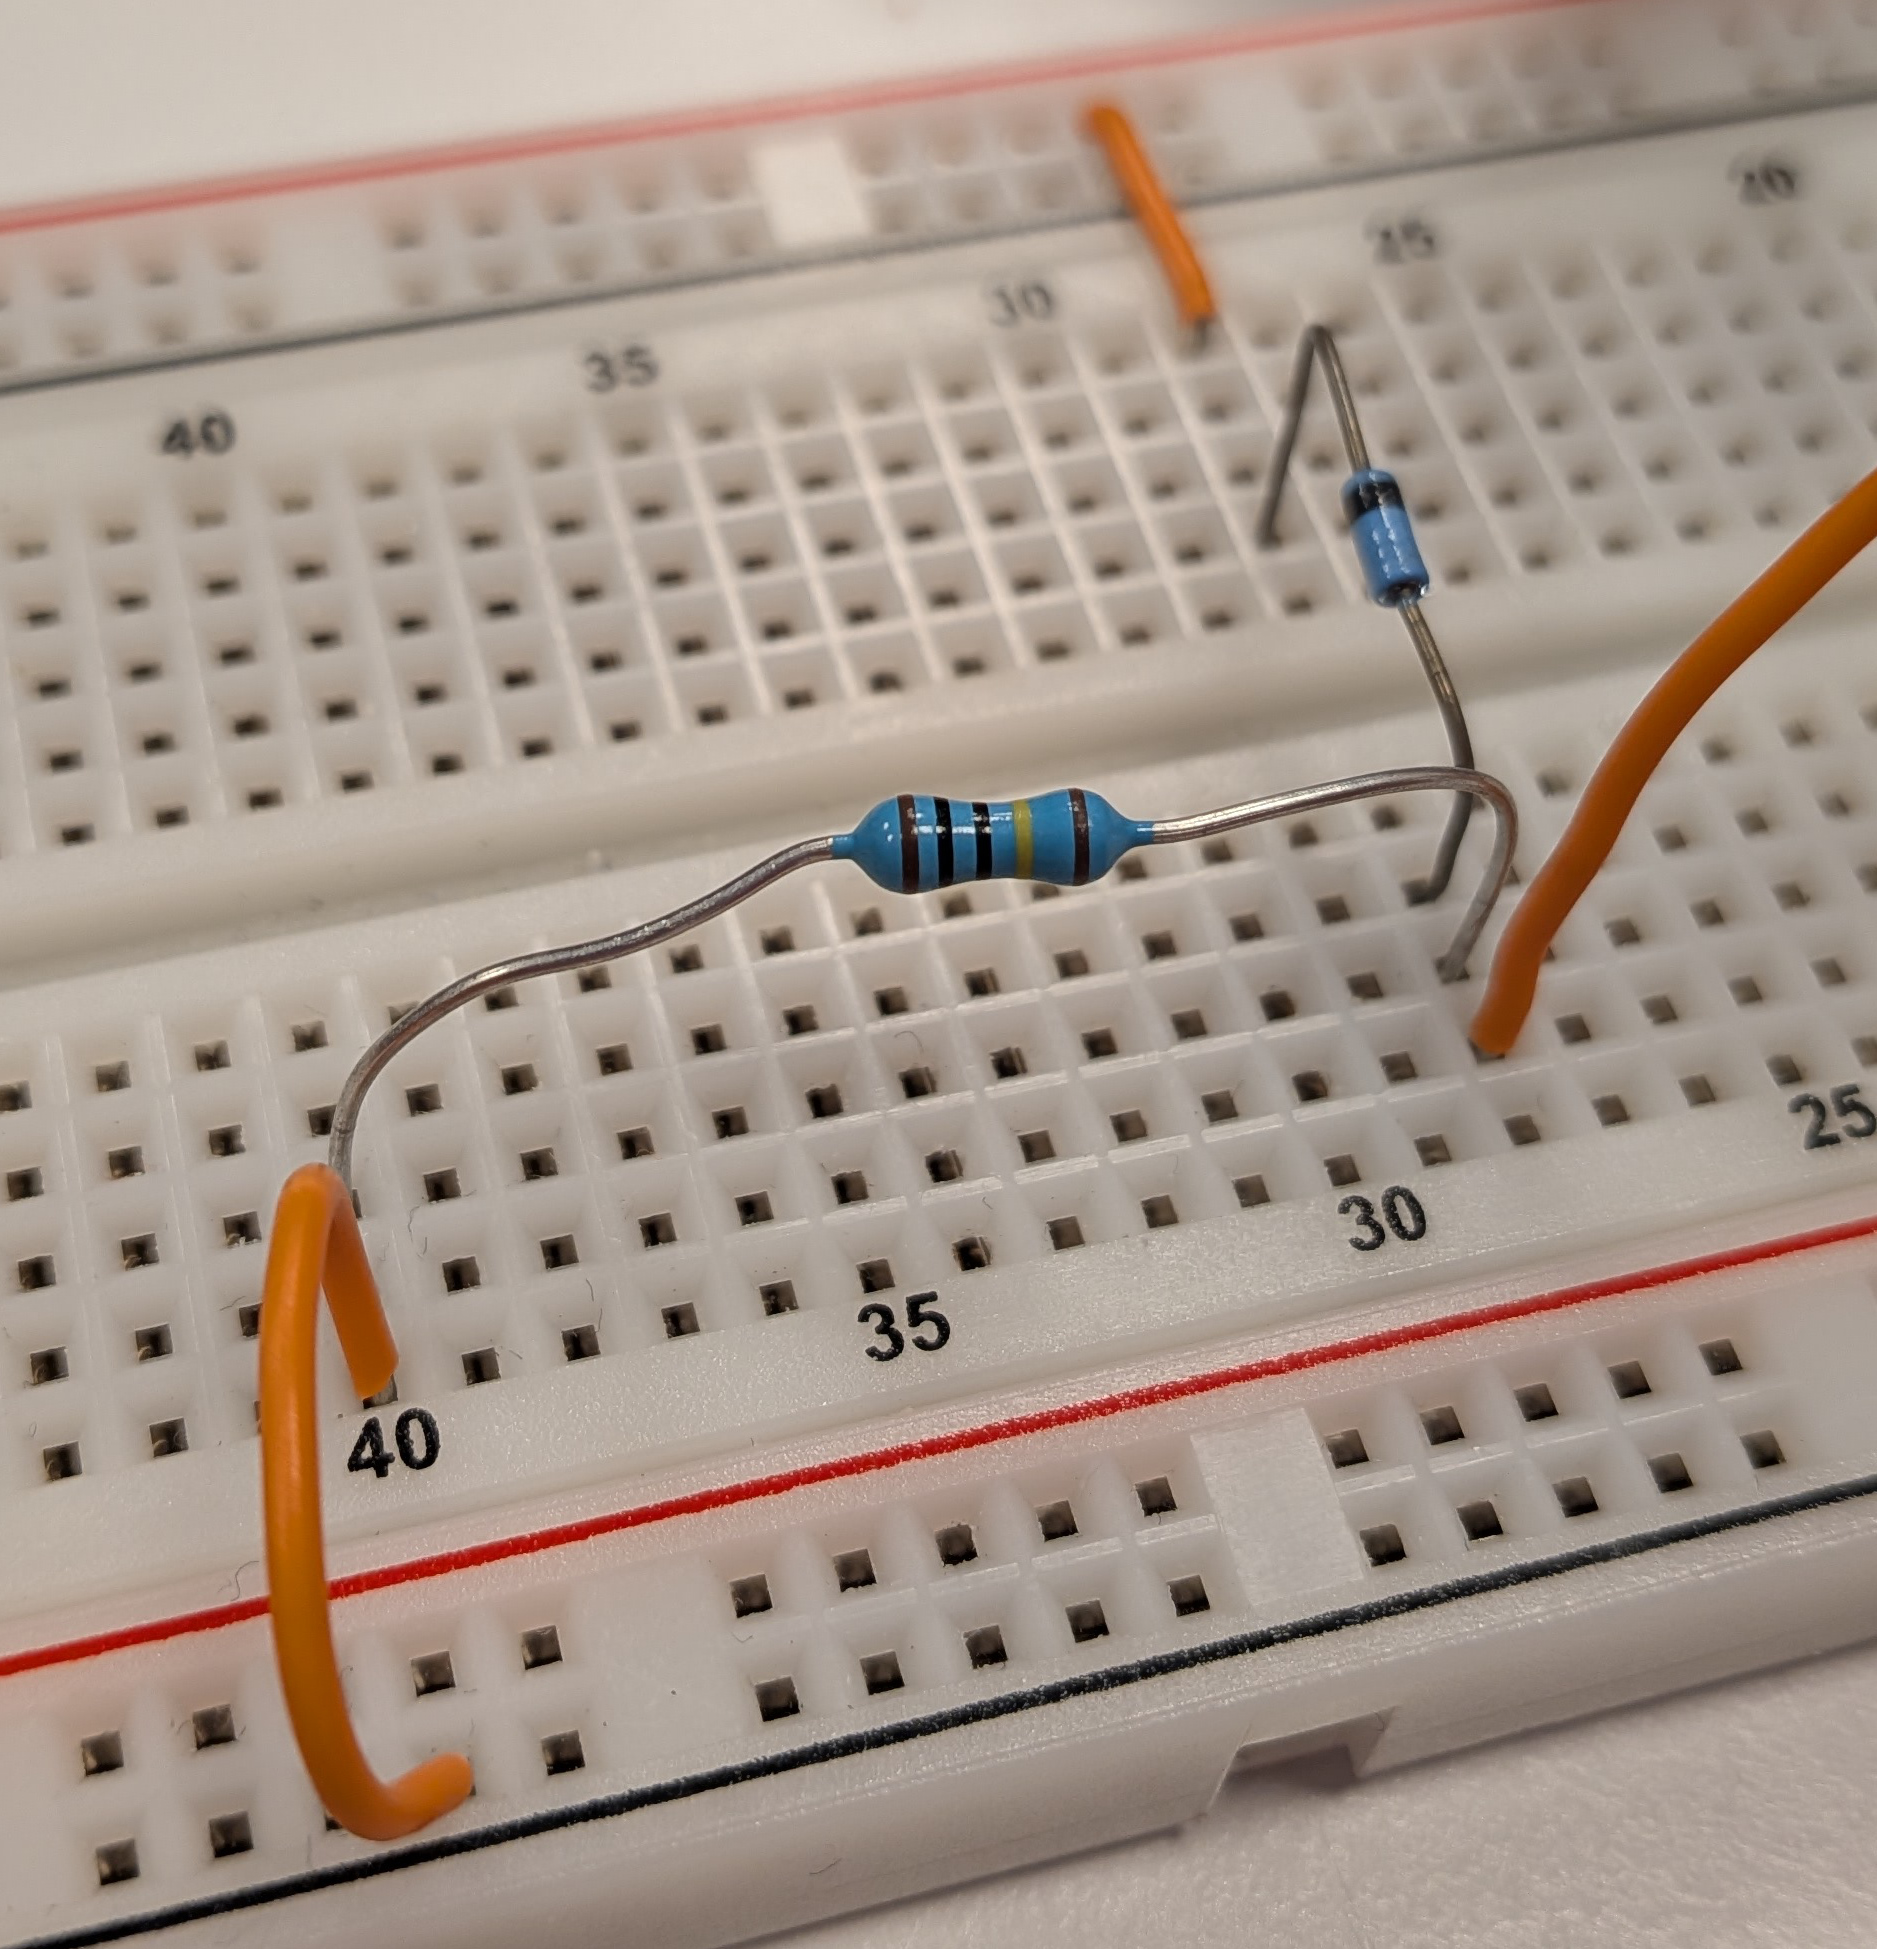
\includegraphics[width=\textwidth]{Part3.jpg}
    \caption{Part 3 circuit}
    \label{fig:Part3}
\end{figure}

\clearpage

%================  TABLE  =========================================================%

% Table generated by Excel2LaTeX from sheet 'Sheet1'
\begin{table}[htbp]
  \centering
  \caption{Reverse-bias measurments}
    \begin{tabular}{|l|rl|}
    \hline
    \(E\) (Measured) & 20.03 & V \bigstrut\\
    \hline
    \(R_M\) (Assumed) & 10    & M\Omega \bigstrut\\
    \hline
    \(R\) (Measured) & 1002.5 & k\Omega \bigstrut\\
    \hline
    \(V_R\) (Measured) & 6.2   & mV \bigstrut\\
    \hline
    \(I_S\) (Calculated) & 6.805 & nA \bigstrut\\
    \hline
    \(R_{DC}\) (Calculated) & 2942.71 & M\Omega \bigstrut\\
    \hline
    \end{tabular}%
  \label{tab:Part3}%
\end{table}%

It looks as if the values for \(I_S\) and \(R_{DC}\) miss by an order of magnitude or two as the calculated reverse-bias resistance often leads to values between hunders of \(\SI{}{\kilo\ohm}\) and up to a hundred \(\SI{}{\mega\ohm}\). The inherent inaccuracies in the measurments are probably the cause of this magnitudinal error.
% #endregion

%================  SECTION  =======================================================%

\section{Part 4 - LED characteristics}
% #region
This part is about testing the characteristics of LED's. 

%================  SINGLE FIGURE  =================================================%

\begin{figure}[h]
    \centering
    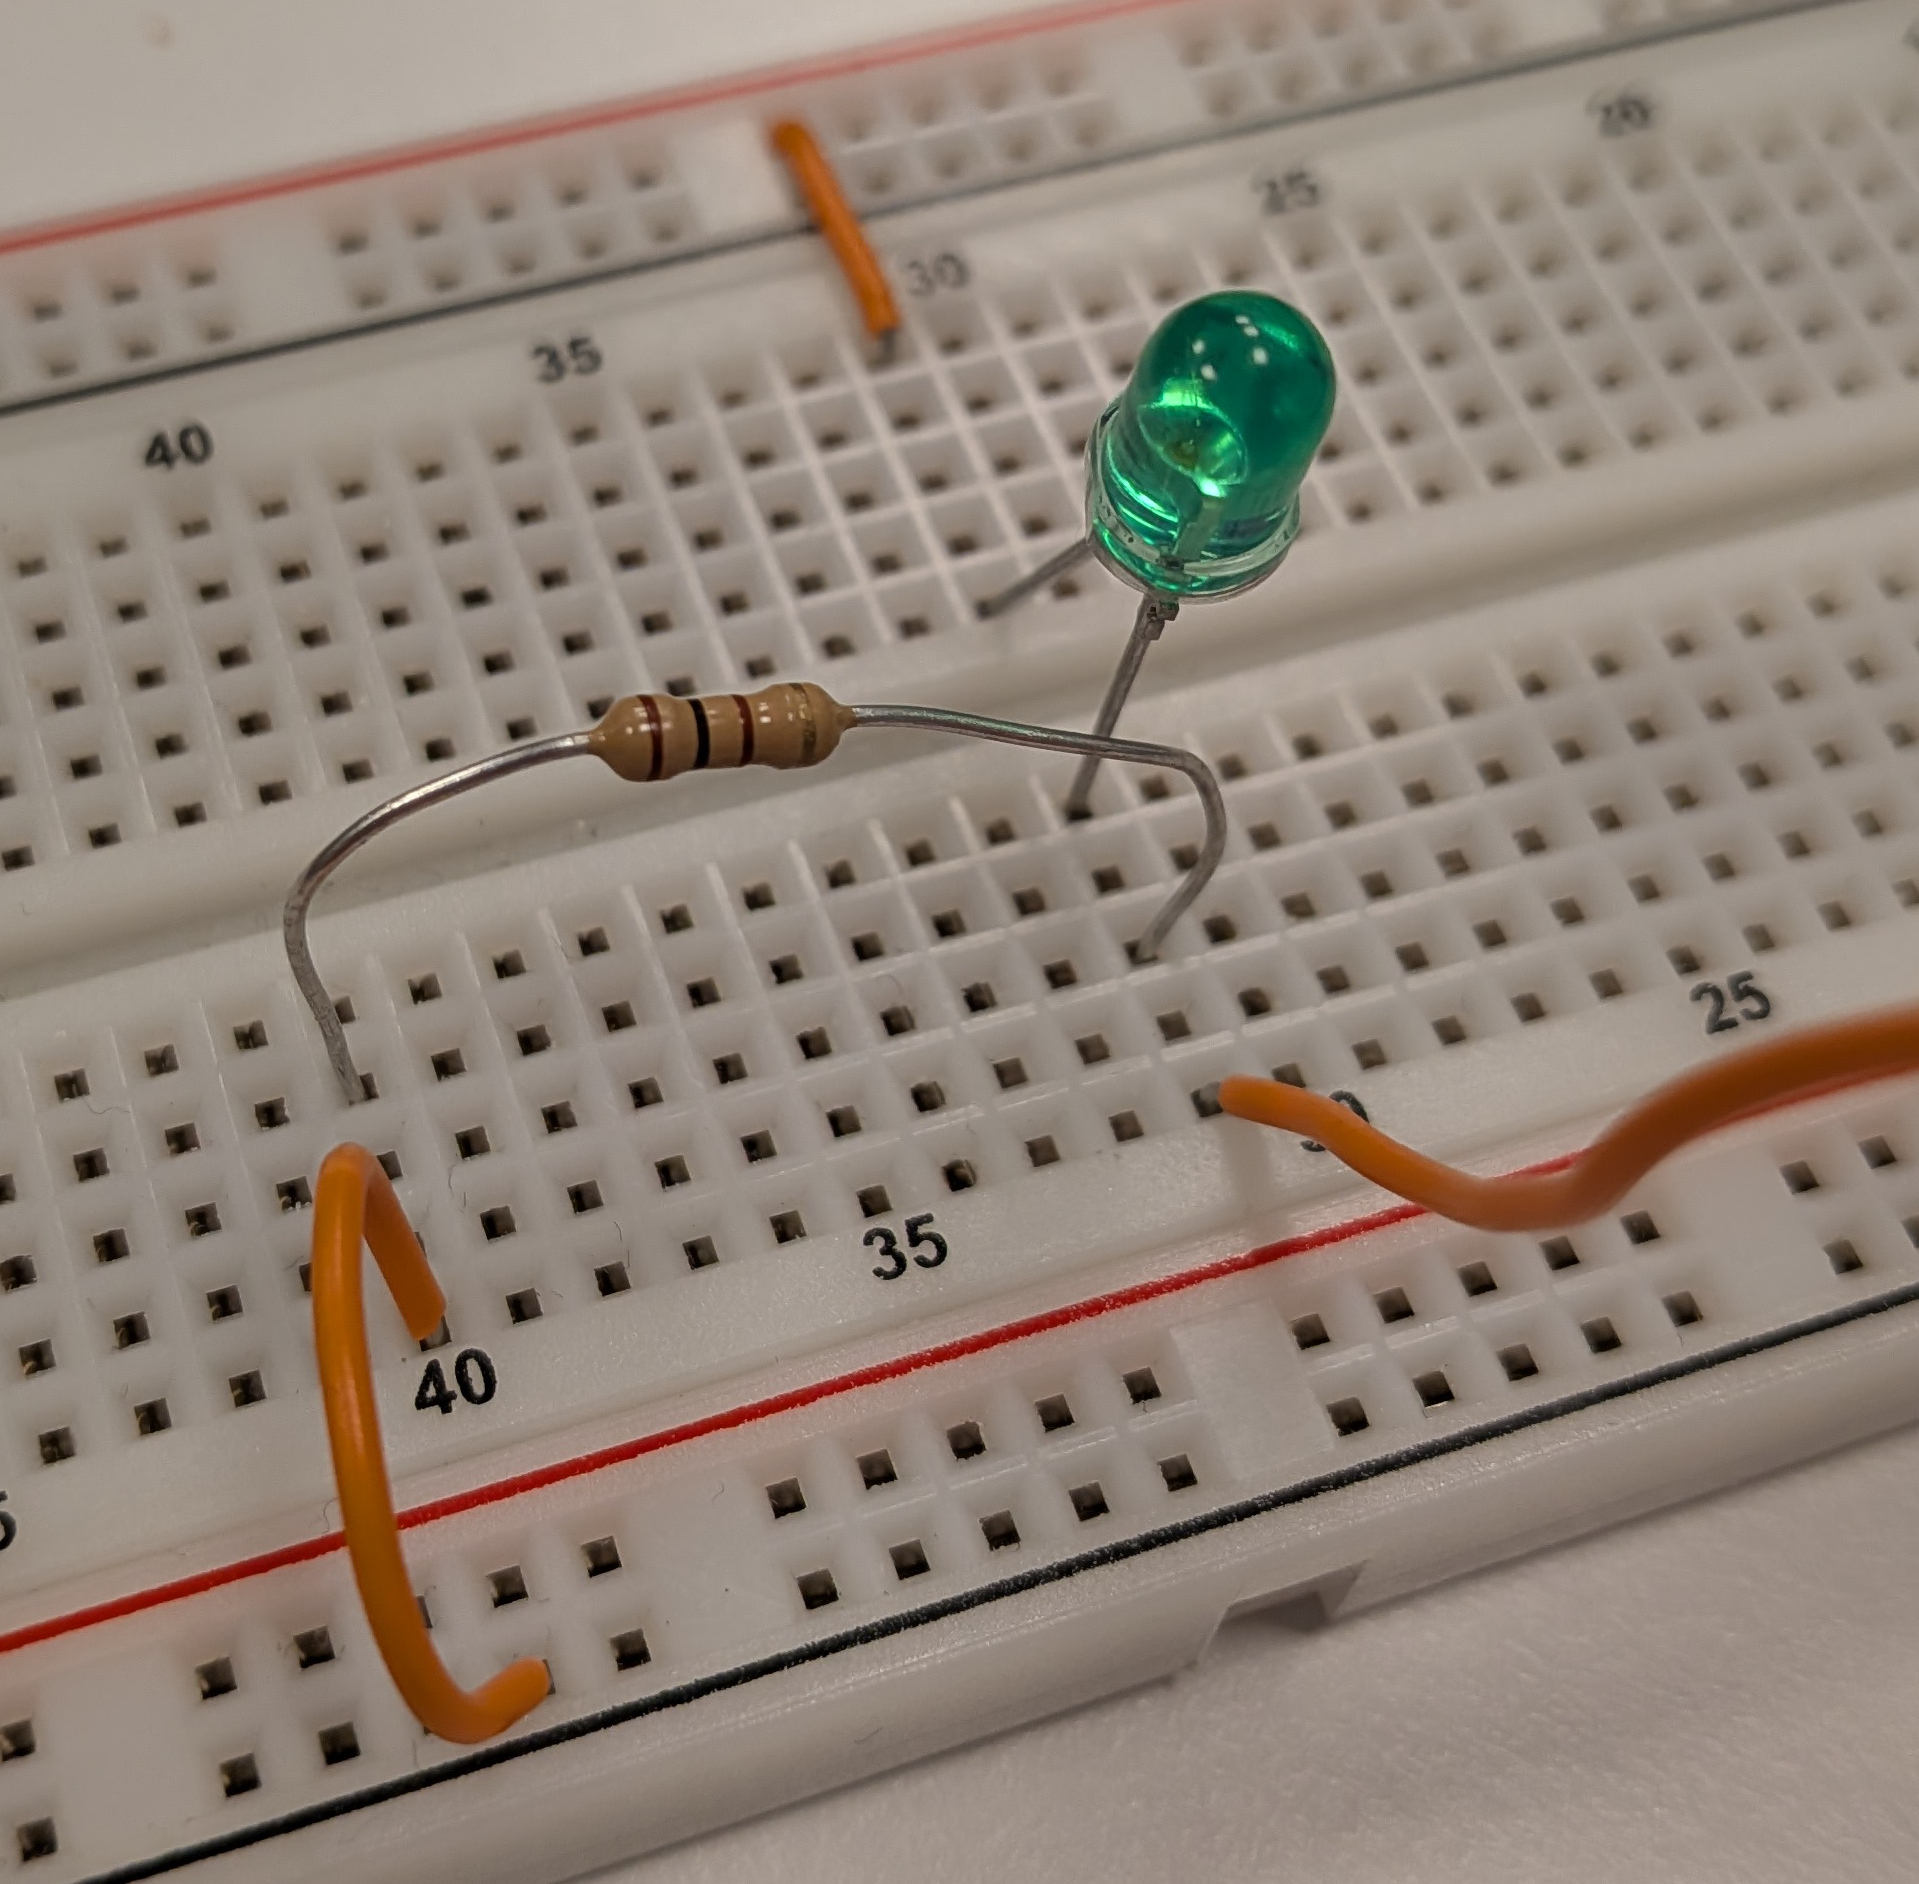
\includegraphics[width=\textwidth]{Part4.jpg}
    \caption{Part 4 circuit}
    \label{fig:Part4}
\end{figure}

First the circuit was connected and then the voltage supply was slowly ramped up. when first light appeared the value was recorded. Although hard to see, in Figure~\ref{fig:FirstLight} there is a very faint sub-lumen light emitting from the diode. Then the supply was ramped up intill brightness leveled out at a bright level and values was recorded again.

\clearpage

%================  TABLE  =========================================================%

% Table generated by Excel2LaTeX from sheet 'Sheet1'
\begin{table}[htbp]
  \centering
  \caption{LED measurments}
    \begin{tabular}{|l|rl|rl|}
    \hline
    Measurments & \multicolumn{2}{c|}{First light} & \multicolumn{2}{c|}{Bright} \bigstrut\\
    \hline
    \(V_D\) (Measured)   & 1.787   & V   & 2.185  & V \bigstrut\\
    \hline
    \(V_R\) (Measured)   & 17.8    & mV  & 3.632  & V \bigstrut\\
    \hline
    \(I_D\) (Calculated) & 179.980 & μA  & 36.724 & mA \bigstrut\\
    \hline
    \end{tabular}%
  \label{tab:part4}%
\end{table}%

\vspace{2em}

%================  MULTI-FIGURE (WITH SUBFIGURES)  ================================%

\begin{figure}[h]
    \centering
    \begin{subfigure}[t]{0.49\textwidth}
        \centering
        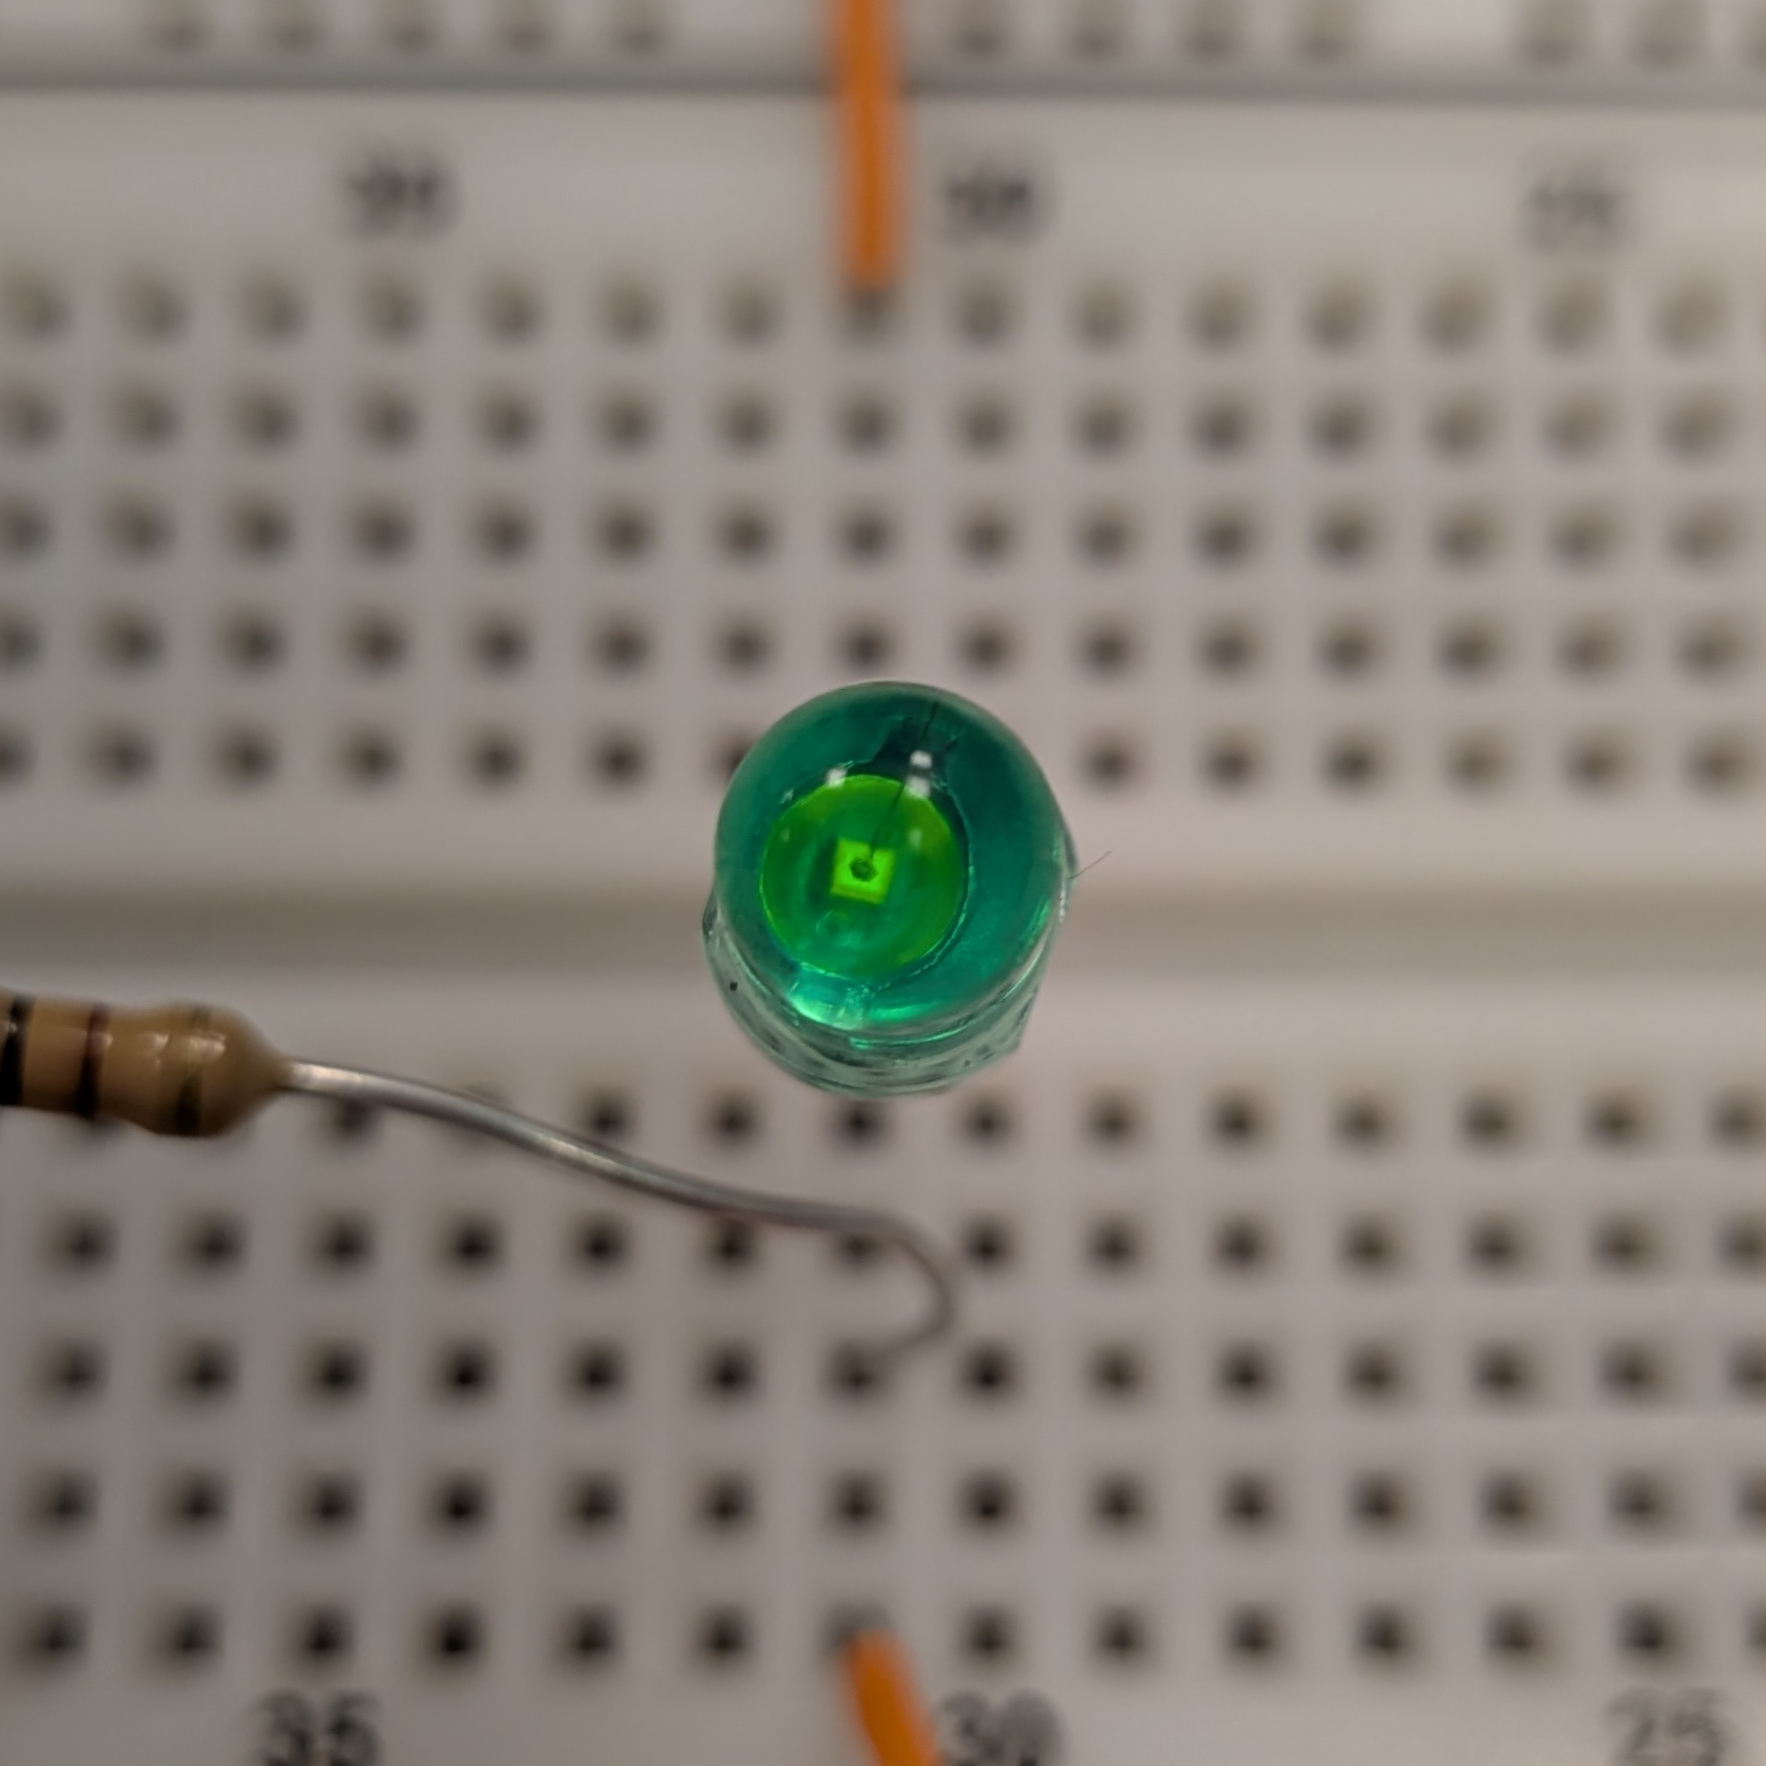
\includegraphics[width=0.9\textwidth]{Part4_FirstLight.jpg}
        \subcaption{First light}
        \label{fig:FirstLight}
    \end{subfigure}
    \hfill
    \begin{subfigure}[t]{0.49\textwidth}
        \centering
        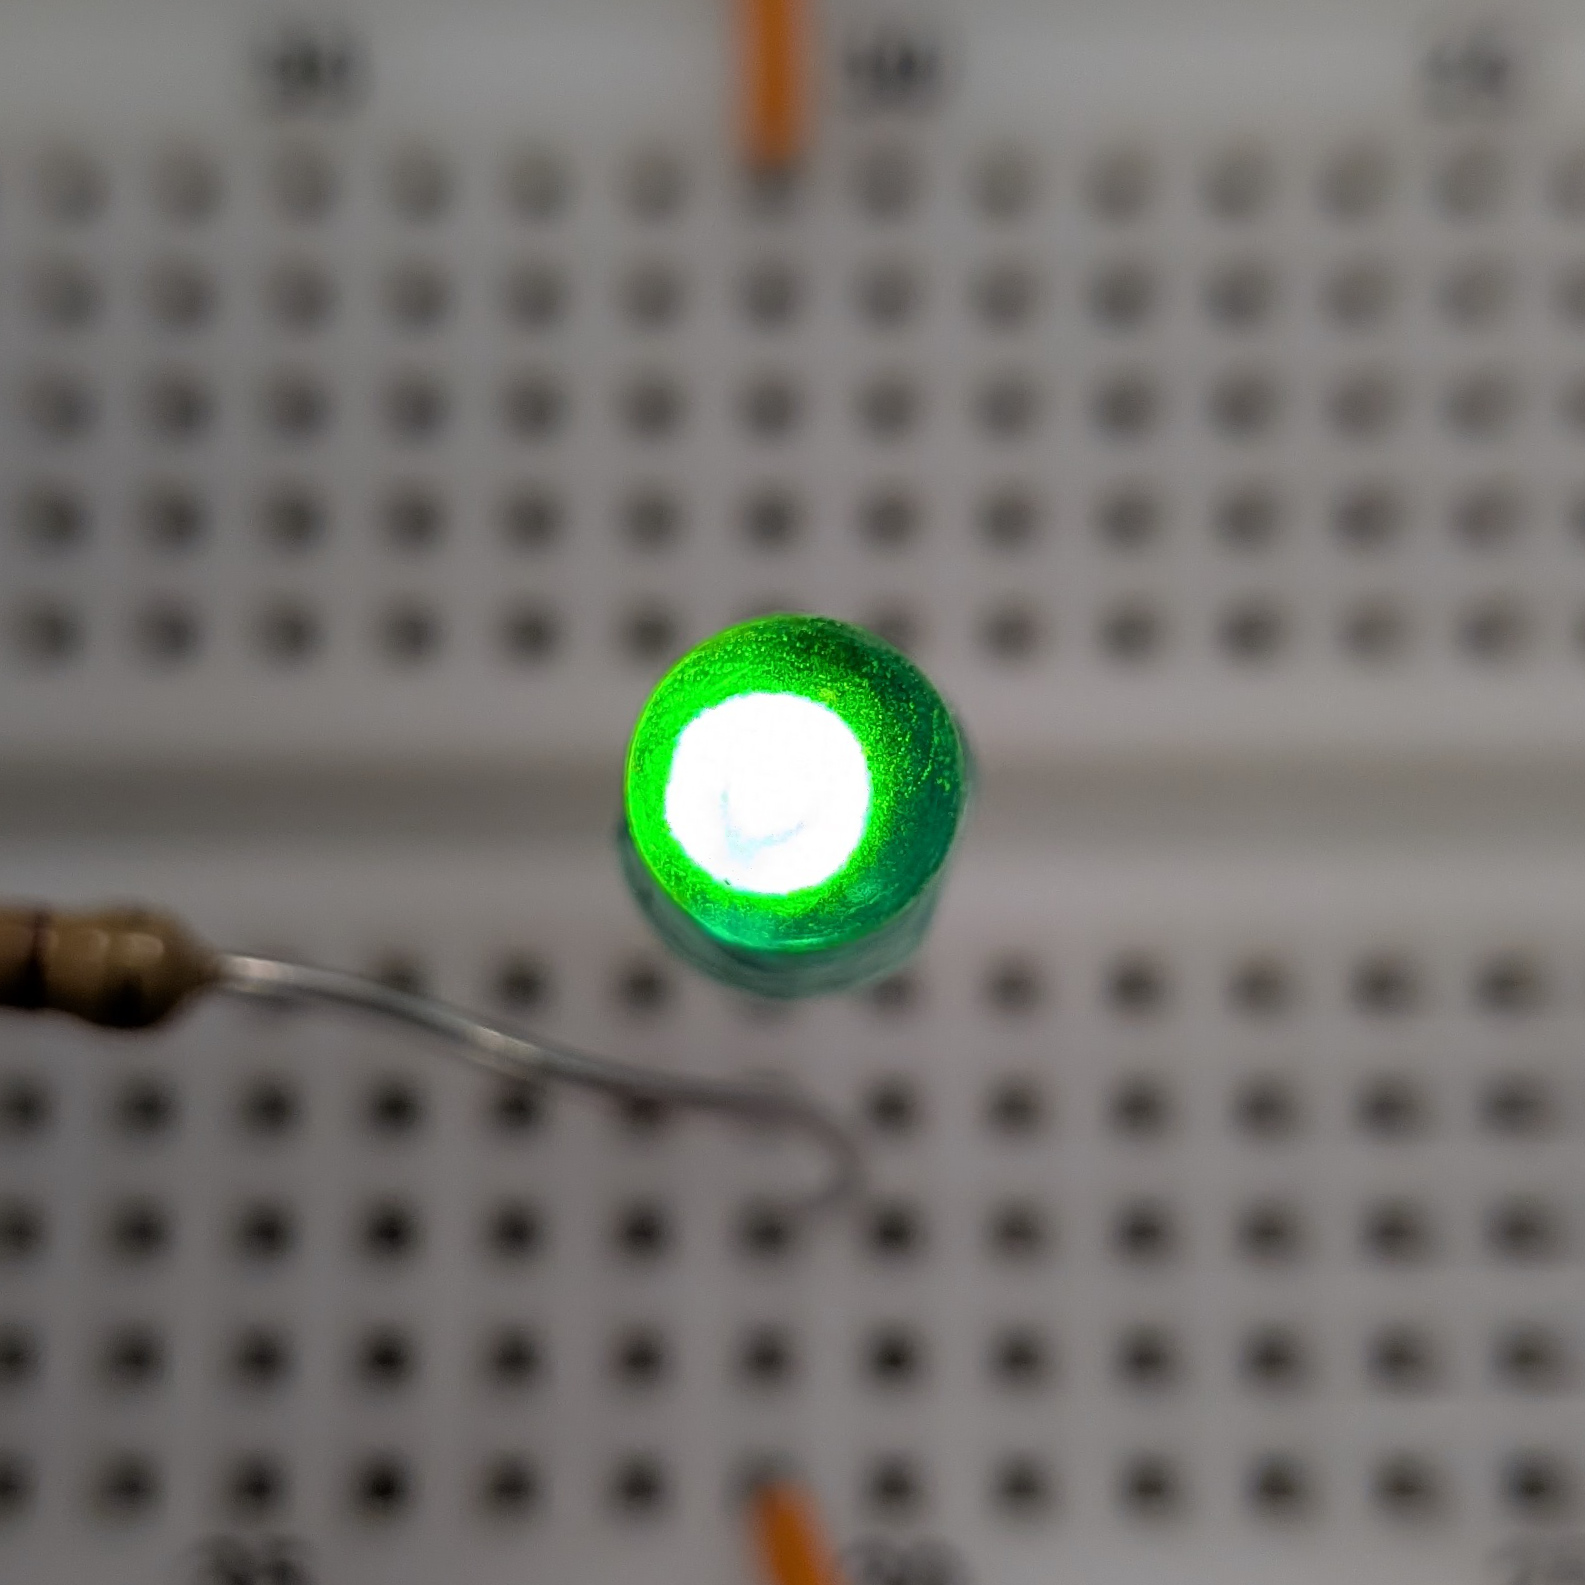
\includegraphics[width=0.9\textwidth]{Part4_FullyOn.jpg}
        \subcaption{Bright}
        \label{fig:Bright}
    \end{subfigure}
    \caption{Part 4 circuit}
    \label{fig:Part4States}
\end{figure}

Then multiple data points was collected for differnt input voltages, and the results are listed below in Teble~\ref{tab:LED} and then graphed.

%================  TABLE  =========================================================%

% Table generated by Excel2LaTeX from sheet 'Sheet1'
\begin{table}[htbp]
  \centering
  \caption{LED values}
  \resizebox{\textwidth}{!}{%
    \begin{tabular}{|l|r|r|r|r|r|r|r|}
      \hline
      \(E\) (V) & 0.000 & 1.033 & 2.008 & 3.008 & 4.002 & 5.010 & 6.040 \bigstrut\\
      \hline
      \(V_D\) (V) & 0.000 & 1.032 & 1.860 & 1.987 & 2.066 & 2.135 & 2.201 \bigstrut\\
      \hline
      \(V_R\) (V) & 0.000 & 0.000 & 0.146 & 1.019 & 1.934 & 2.875 & 3.840 \bigstrut\\
      \hline
      \(I_D\) (mA) & 0.000 & 0.000 & 1.480 & 10.303 & 19.555 & 29.070 & 38.827 \bigstrut\\
      \hline
    \end{tabular}%
  }
  \label{tab:LED}%
\end{table}


% #endregion
%================  SECTION  =======================================================%

\section{Part 5 - Zener characteristics}
% #region

% #endregion



\end{document}